\section{Diagrammes UML de Connect Four}


\begin{figure}[H]
    \centering
    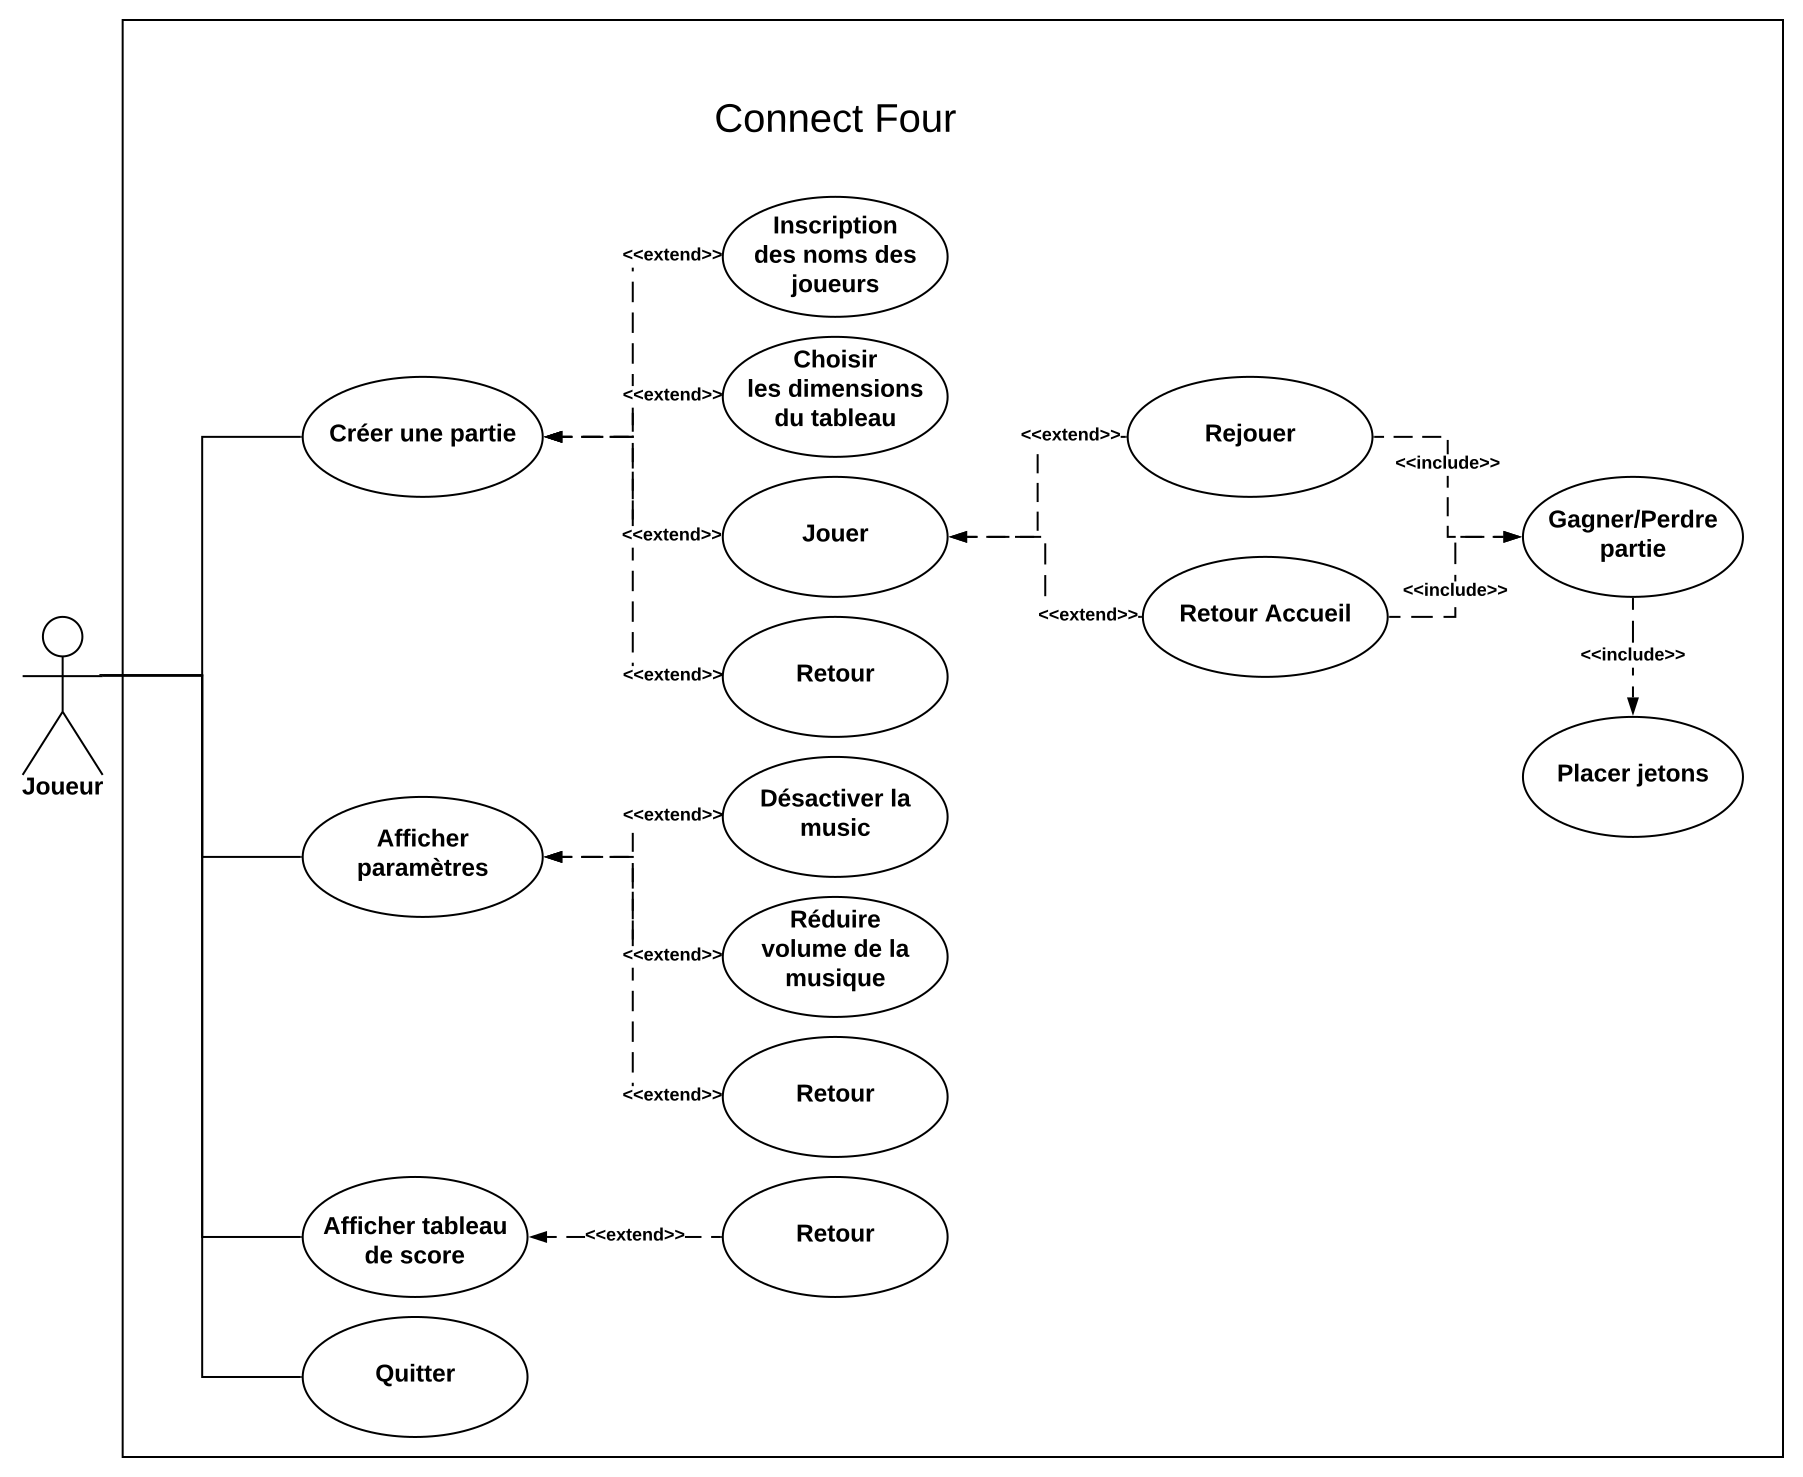
\includegraphics[width=6in]{img/cas}
    \caption{Diagramme de cas d’utilisation UML de haut niveau de Connect Four}
\end{figure}

\begin{figure}[H]
    \centering
    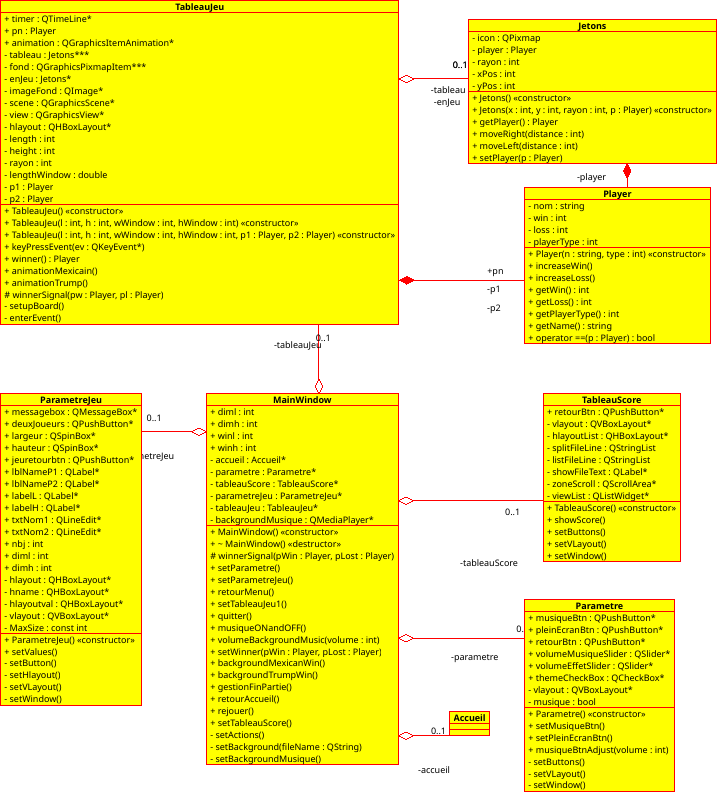
\includegraphics[width=6in]{img/classes}
    \caption{Diagramme de classe de Connect Four}
\end{figure}

\section{Captures d’écrans}

\begin{figure}[H]
    \centering
    
\includegraphics[width=6in]{img/1}
    \caption{Écran 1}
\end{figure}

\begin{figure}[H]
    \centering
    
\includegraphics[width=6in]{img/2}
    \caption{Écran 2}
\end{figure}

\begin{figure}[H]
    \centering
    
\includegraphics[width=6in]{img/3}
    \caption{Écran 3}
\end{figure}

\begin{figure}[H]
    \centering
    
\includegraphics[width=6in]{img/4}
    \caption{Écran 4}
\end{figure}

\section{But, fonctionnement et guide d'usager de Conect Four}

Le but de cette application est de permettre à deux personnes de jouer au jeu puissance~4 sans l’usage de leurs mains.

De plus, la forme finale de l’application permettra de jouer contre un ordinateur à niveau de difficulté variable.
Il est possible de choisir les dimension du tableau de jeu, les noms des participants et, si l’on veut, la musique et les effets sonores.

La base de l’application est un QMainWindow ou l’on change le central widget selon ce qui est sélectionné par l’usager.
Pour le tableau de jeu, la méthode QGraphicsScene a été utilisée pour pouvoir ajouter dynamiquement des éléments à la fenêtre de jeu.

\section{Ergonomie et amélioration}

\section{Plan de tests de Connect Four}

\begin{table}[H]
    \centering
    \caption{Plan de tests de l'interface graphique}
    \begin{tabular}{p{0.25in}p{2.5in}p{0.5in}p{2.5in}}
        \hline
        \bfseries Test & \bfseries Description et résultats & \bfseries Passé & \bfseries Justification \\
        \hline\hline
        1 & Nombre d'élément dans le menu inférieur à 7 & Oui & Tous les menus ont moins de 7 éléments \\
        2 & L'utilisateur peux revenir au menu principal en tout temps. & Non & Certains écrans ne contiennent pas bouton de retour à l'écran principal.\\
        3 & Dans le tableau de score, les scores sont aligné lorsque les noms ont 6 charactères. & Oui & Les scores sont allignés.\\
        4 & Dans le tableau de score, chaque noms n'apparait qu'une seule fois. & Non & Les nom peuvent apparaître plusieur fois.\\
        \hline
    \end{tabular}
\end{table}

\begin{table}[H]
    \centering
    \caption{Plan de tests de l'application}
    \begin{tabular}{p{0.25in}p{2.5in}p{0.5in}p{2.5in}}
        \hline
        \bfseries Test & \bfseries Description et résultats & \bfseries Passé & \bfseries Justification \\
        \hline\hline
        1 & On peux déplacer le pion de gauche à droite & Oui & Le pion se déplace de gauche à droite \\
        2 & Le pion ne peux pas aller à l'extérieur du plateu & Oui & Le déplacement du pion est limité à la largeur du plateau de jeu \\
        3 & Le jeton tombe à l'endroit attendu lorsque qu'on appuie sur la bare d'espacement & Oui & Le pion tombe au bon endroit \\
        4 & Lorsque 4 jetons sont aligné, le bon gagnant est déclaré. & Oui & Le bon gagnant est déclaré vaiceur à la fin de la partie.\\
        5 & Lorsqu'il n'est plus possible d'ajouter un jeton (le tableau est plein), l'utilisateur devrait pouvoir recommencer une autre partie.& Non & L'utilisateur reste bloqué dans le tableau.\\
        \hline
    \end{tabular}
\end{table}
